\section{Bedienung}
    Das Spiel wird mit vier Tasten gesteuert.
    Dabei wird der Cursor mit der linken und der rechten Taste, jeweils um eine eine Spalte in die gewünschte Richtung bewegt.
    Mit der unteren Taste wird ein Stein, an der aktuellen Cursorposition, in die Spalte geworfen.
    Über die Resettaste kann das komplette Spiel zurückgesetzt werden. Spieler 1 wäre nun wieder am Zug.
    \begin{figure}[H]
        \centering
        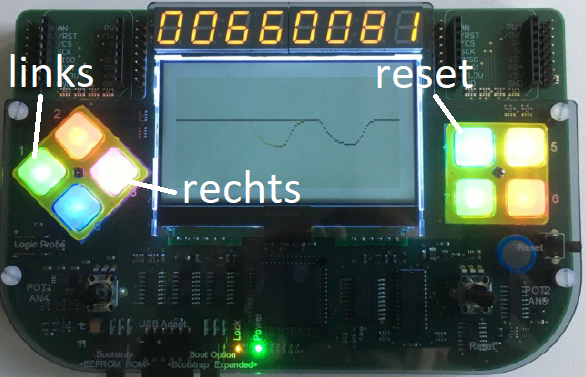
\includegraphics[scale=0.5]{img/board.png}    
        \caption{Board}
        \label{fig:board}
    \end{figure}

\section{Ausgabe}
    \subsection{Spielstart}
        Nach erfolgreichem Programmstart wird das leere Spielfeld in der Mitte des LCD's angezeigt.
        Links davon befindet sich ein Textfeld \textit{turn}, welches den Namen des Spielers anzeigt, der zurzeit dran ist.
        Beim Programmstart sowie beim Zurücksetzen des Spieles startet immer \textit{Spieler 1}.
        Unter dem Spielfeld ist der Cursor zu sehen, der zum Start des Spieles auf die mittlere Spalte zeigt.

        \begin{figure}[H]
            \centering
            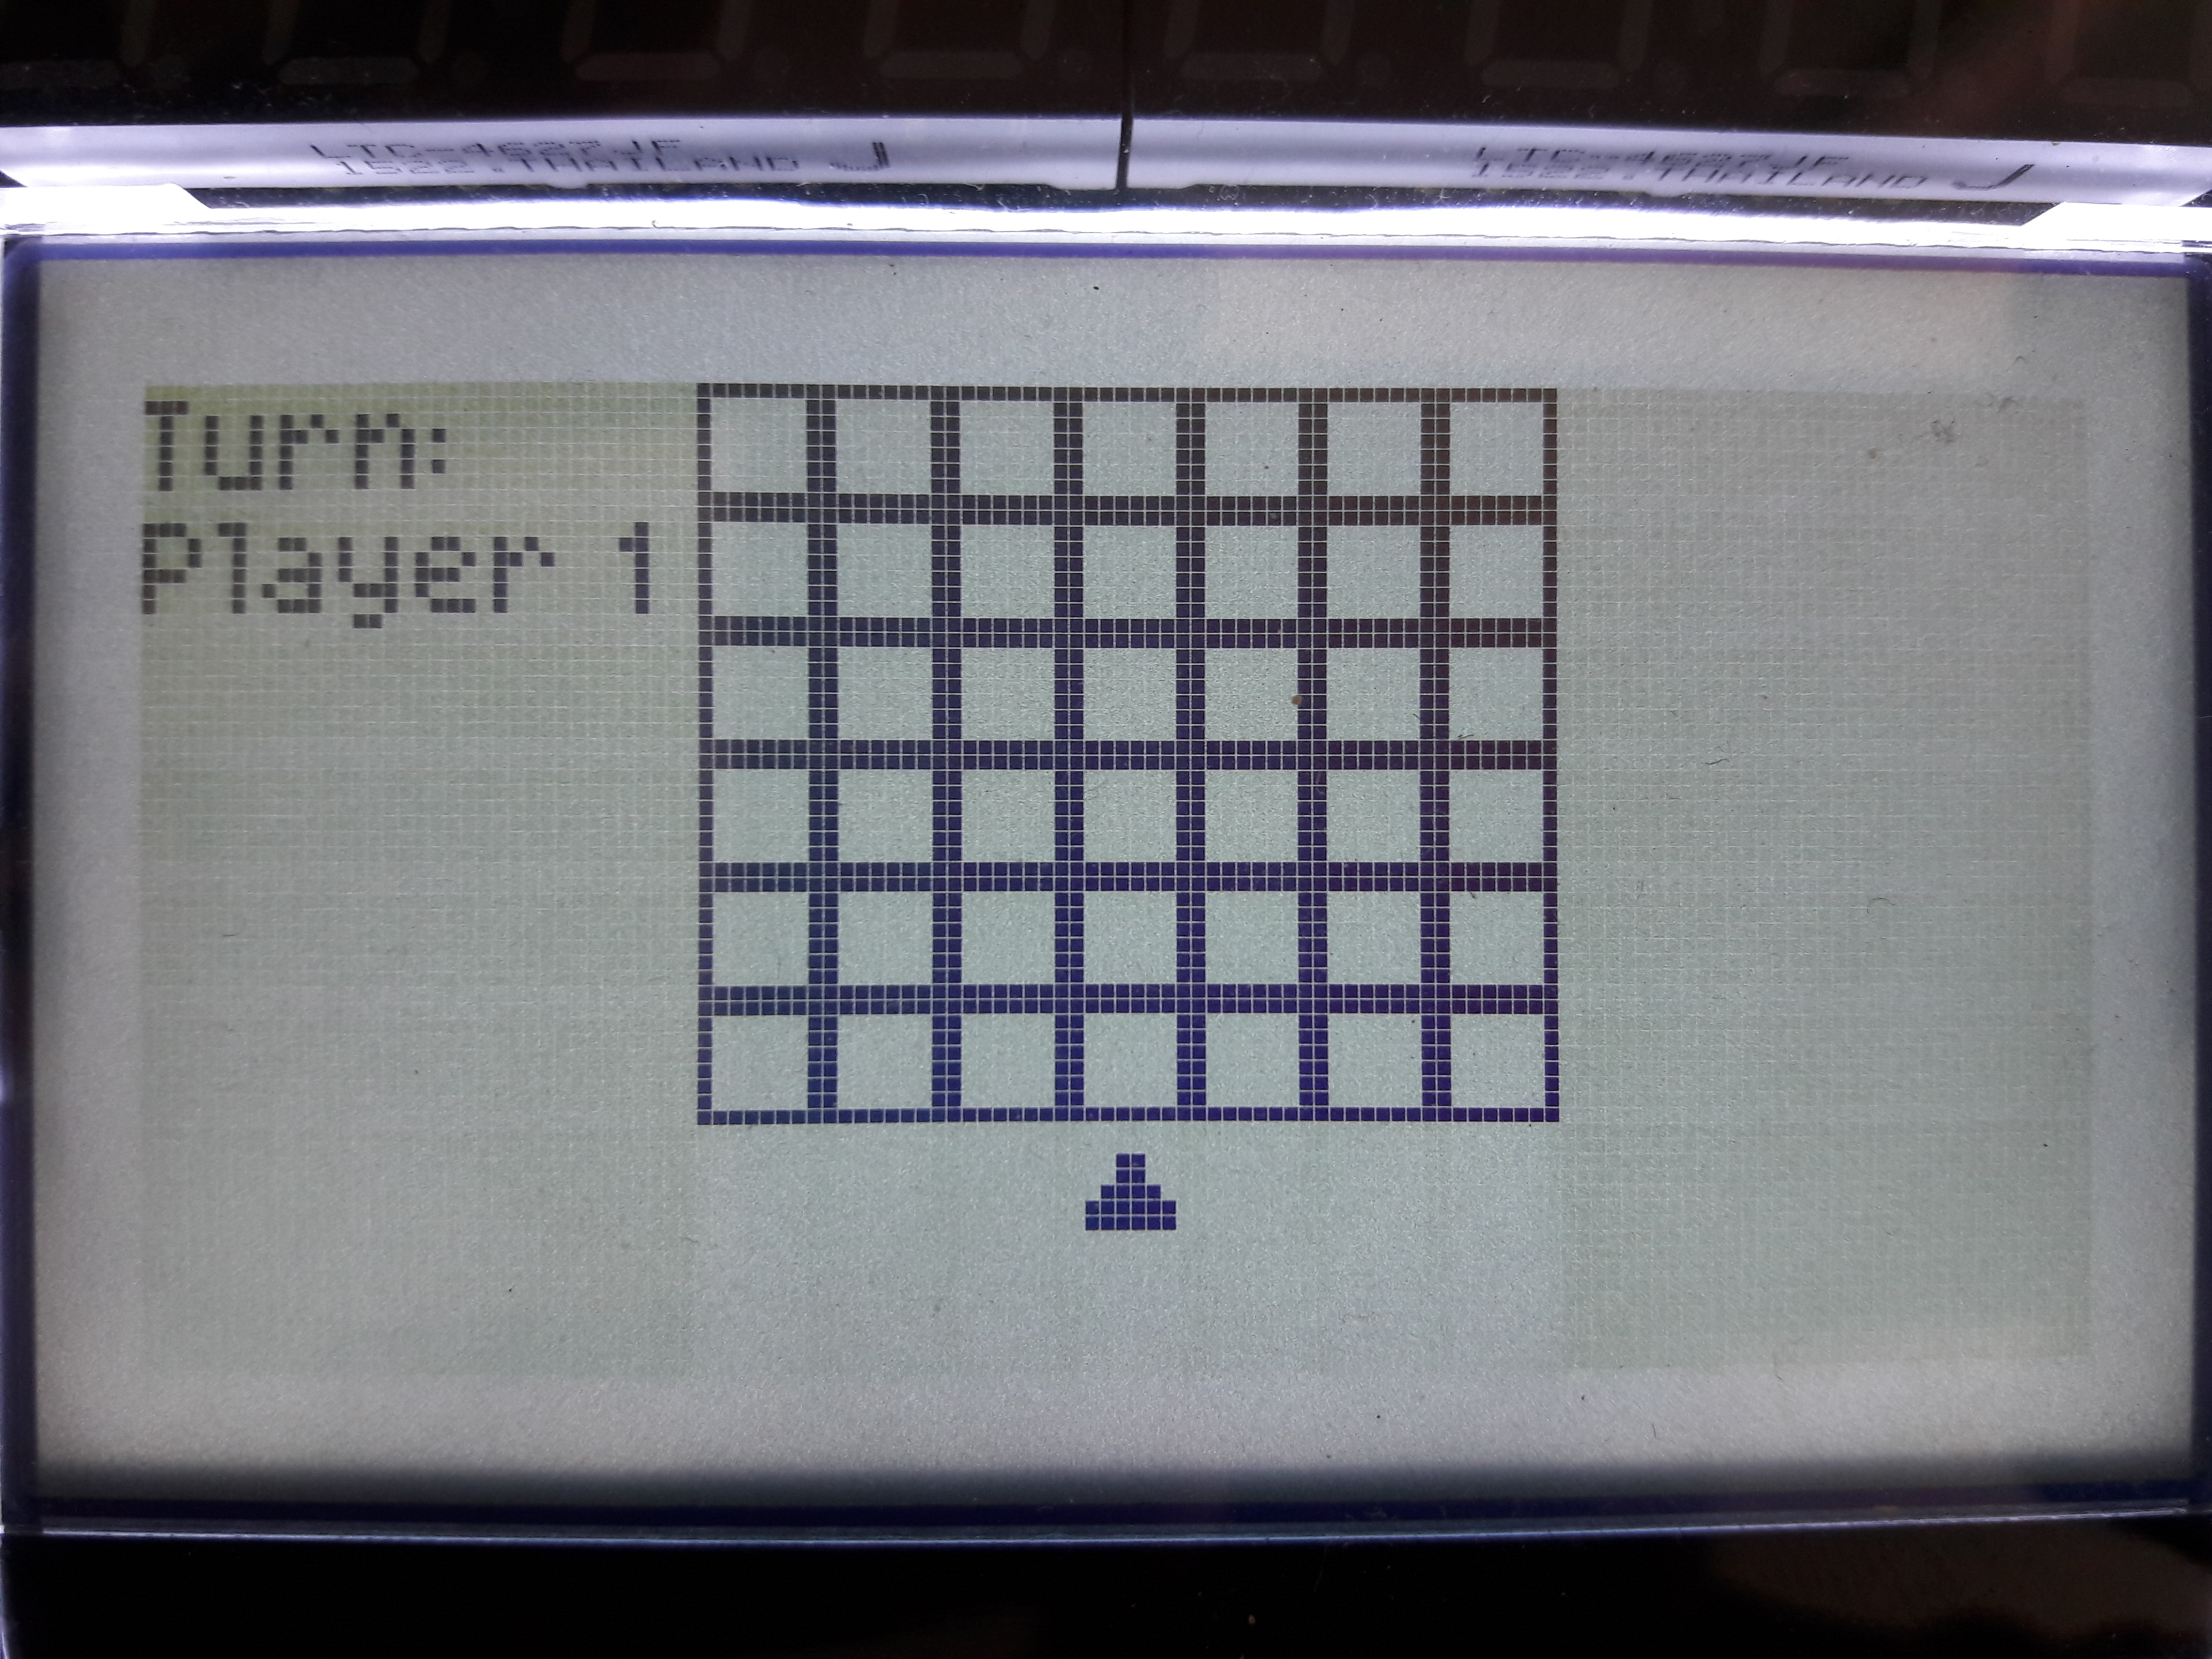
\includegraphics[width=\textwidth]{img/start.jpg}    
            \caption{Spielstart}
        \end{figure}

    \subsection{Spielende}
        Falls ein Spieler gewonnen hat, wird unter dem Spielfeld der gewinnende Spieler angezeigt.
        Zusätzlich ist die Eingabe blockiert und das Spiel lässt sich nur mit den Resetbutton zurücksetzen.

        \begin{figure}[H]
            \centering
            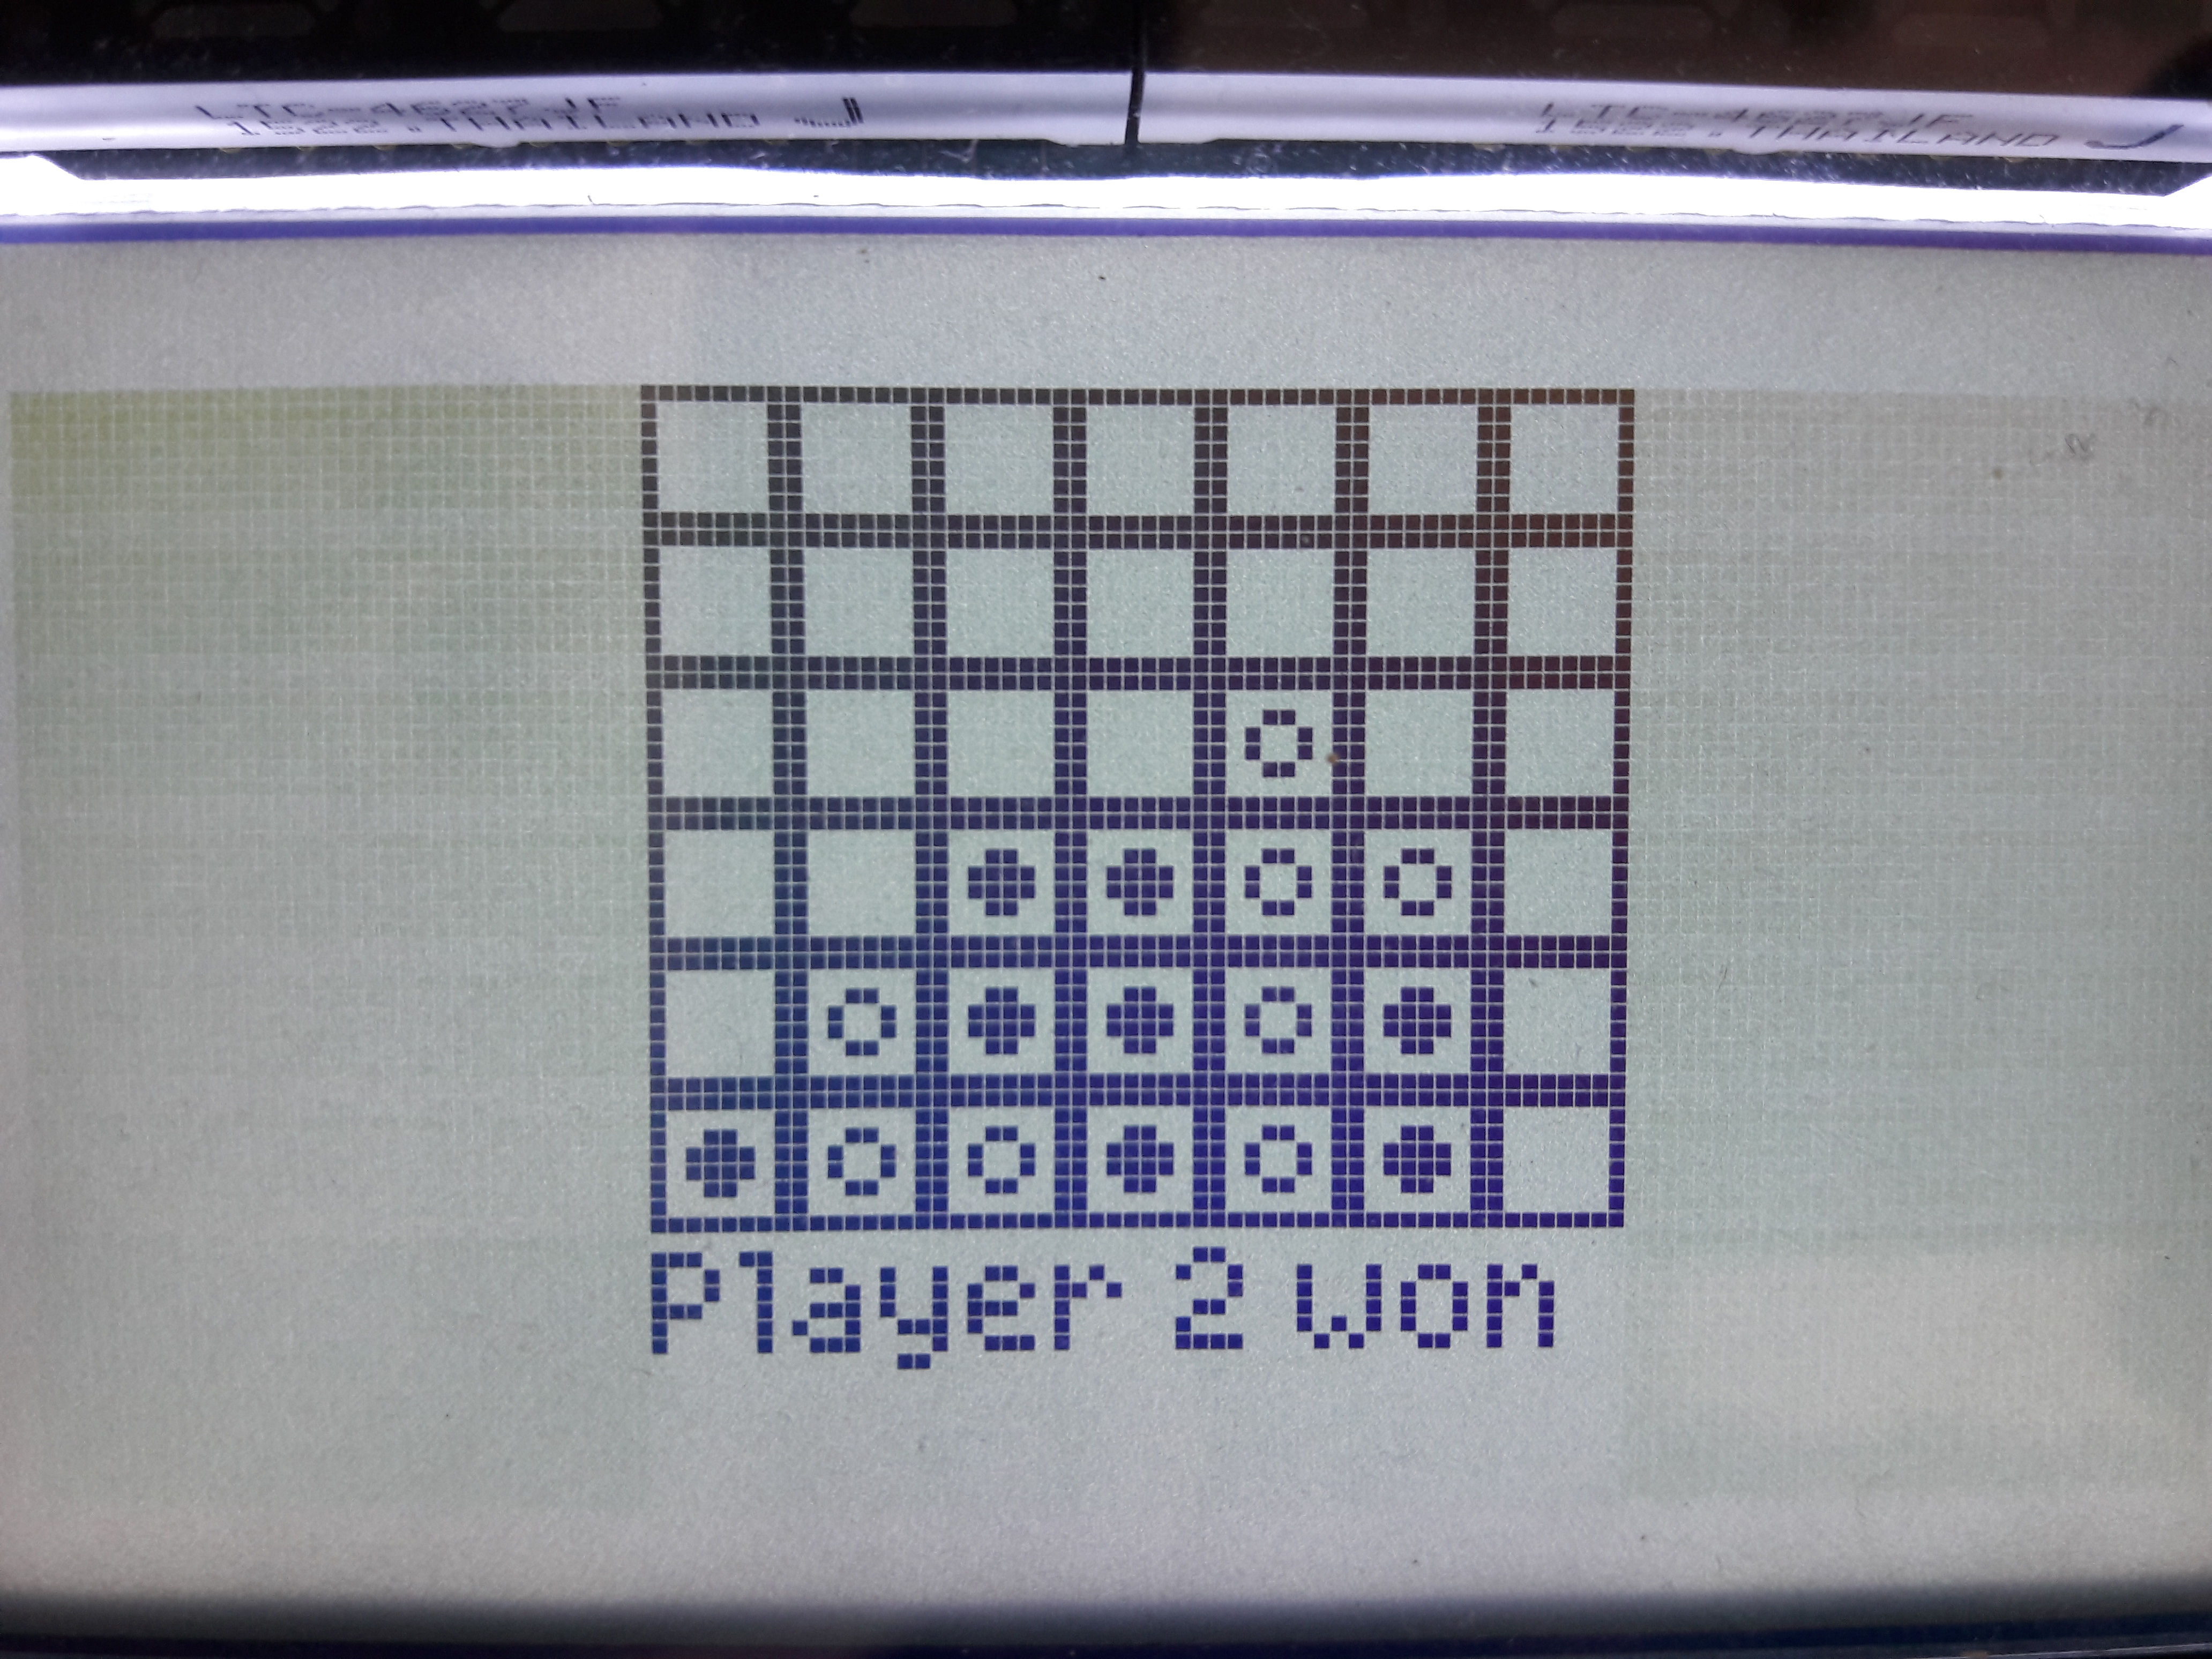
\includegraphics[width=\textwidth]{img/player_2_won.jpg}    
            \caption{Spielende}
        \end{figure}




